\documentclass{scrartcl}

% TODO: rausfinden was mit den 2 Termen in der letzten Glg passiert
% TODO: Formel Layout verbessern (Abstände etc.) -> wenn alles andere passt
% TODO: Alle nicht referenzierten Gleichungen mit *
% TODO: Wichtige Gleichungen/Ergebnisse einrahmen?

% packages
\usepackage[utf8]{inputenc}
\usepackage{amsmath}
\usepackage{cancel}
\usepackage[left=25mm,right=25mm,top=3cm,bottom=3cm]{geometry}
\usepackage{physics}
\usepackage{mathrsfs}
\usepackage{tikz}
\usepackage[small,bf]{caption}

\usetikzlibrary{arrows.meta}
\usetikzlibrary{calc}

% settings
\setlength{\parindent}{0pt}
\setlength{\parskip}{6pt}
\allowdisplaybreaks[2]

% commands for vectors
\renewcommand{\vec}[1]{\boldsymbol{#1}}
\newcommand{\uv}[1]{\hat{\vec{#1}}}
\newcommand{\bnabla}{\vec{\nabla}}

% short commands for position vectors r and R
\newcommand{\rv}{\vec{r}}
\newcommand{\rvdot}{\dot{\rv}}
\newcommand{\rvgc}{\vec{R}} % guiding center position
\newcommand{\rgc}{R}

% short commands for phase space vector pi
\newcommand{\pid}{\dot{\pi}}
\newcommand{\pit}{\tilde{\pi}}
\newcommand{\pitd}{\dot{\tilde{\pi}}}
\newcommand{\pivd}{\dot{\vec{\pi}}}
\newcommand{\pivt}{\tilde{\vec{\pi}}}
\newcommand{\pivtd}{\dot{\tilde{\vec{\pi}}}}

% short commands for phase space Lagrangian
\newcommand{\lag}{L}
\newcommand{\ham}{H}
\newcommand{\PSL}{\mathcal{L}}
\newcommand{\PSLt}{\tilde{\mathcal{L}}}

% other commands
\newcommand{\subparallel}{{\scriptscriptstyle\parallel}}

% title settings
\title{Derivation of Drift Motion Using a Phase Space Lagrangian Approach}
\subtitle{\vspace{5mm}PHT.512UF Plasma Physics\vfill}
\author{Lukas Grabenwarter}
\date{2018}


\begin{document}

\maketitle
\thispagestyle{empty}
\newpage

\tableofcontents
\thispagestyle{empty}
\newpage

\pagenumbering{arabic}

\section{Phase space Lagrangian mechanics}
\subsection{Review: Lagrangian and Hamiltonian mechanics}\label{sec:review}
The Lagrangian function, shortly called just the \emph{Lagrangian}, for a set of generalized coordinates $\vec{q}$ is defined as the difference of kinetic and potential energy. It is a function of the coordinates and their time derivatives as well as time itself,
\begin{equation*}
\lag(\vec{q},\dot{\vec{q}},t) = T - U   \ .
\end{equation*}
It obeys the Euler-Lagrange equation with respect to each of the coordinates $q_k$,
\begin{equation*}
\dv{t}\pdv{\lag}{\dot{q}_k} - \pdv{\lag}{q_k} = 0 \ .
\end{equation*}
It can be shown that adding a total time derivative to the Lagrangian does not change the form of the Euler-Lagrange equations, which means that a Lagrangian
\begin{equation*}
\lag' = \lag + \dv{f}{t}
\end{equation*}
with an arbitrary function $f$ describes the same system as the original Lagrangian $\lag$.

The conjugate momenta to $\vec{q}$ are defined as
\begin{equation}\label{eq:conj_momenta}
p_k = \pdv{\lag}{\dot{q}_k}
\end{equation}
and the \emph{Hamiltonian} is the Legendre transform of $L$ with respect to $\vec{q}$, which results in
\begin{equation}\label{eq:def_hamiltonian}
\ham(\vec{q},\vec{p},t) = \vec{p}\cdot\dot{\vec{q}}(\vec{q},\vec{p}) - \lag(\vec{q},\dot{\vec{q}}(\vec{q},\vec{p}),t) \ .
\end{equation}
The equations of motion can be obtained directly from the Hamiltonian via Hamilton's equations
\begin{align}
\dot{p}_k &= -\pdv{\ham}{q_k} \ , \nonumber \\
\dot{q}_k &= \pdv{\ham}{p_k} \ . \label{eq:hamilton}
\end{align}
Both the Euler-Lagrange equation and Hamilton's equations are a consequence of \emph{Hamilton's principle}: Among all possible paths the system could follow in phase space, the one it will actually follow is the one that minimizes the action 
\begin{equation*}
S = \int\limits_{t_1}^{t_2}\lag(\vec{q},\dot{\vec{q}},t) \, \dd{t} \ .
\end{equation*}
Therefore both sets of equations can be derived by setting the functional derivative of the action integral to zero,
\begin{equation*}
\delta S = \delta \int\limits_{t_1}^{t_2}\lag(\vec{q},\dot{\vec{q}},t) \, \dd{t} = 0 \ .
\end{equation*}

\subsection{The phase space Lagrangian}\label{sec:phase_space_lagrangian}
Solving \eqref{eq:def_hamiltonian} for $\lag$ gives
\begin{equation}\label{eq:phase_space_lagrangian_def}
\lag = \vec{p}\cdot\dot{\vec{q}} - \ham(\vec{q},\vec{p},t)
\end{equation}
which suggests regarding the Lagrangian as a function of the positions, their derivatives \emph{and} the momenta. Although there is no dependence on $\dot{\vec{p}}$ in \eqref{eq:phase_space_lagrangian_def}, we add a formal dependence to obtain a more general expression, which leads to the so-called \emph{phase space Lagrangian}
\begin{equation}\label{eq:ps_lagrangian_actual_def}
\PSL(\vec{q},\vec{p},\dot{\vec{q}},\dot{\vec{p}},t) := \vec{p}\cdot\dot{\vec{q}} - \ham(\vec{q},\vec{p},t) \ . 
\end{equation}
It can easily be shown that the Euler-Lagrange equations hold for the phase space Lagrangian with respect to any position $q_k$ or momentum $p_k$: For the position variables one obtains directly from \eqref{eq:ps_lagrangian_actual_def}
\begin{align*}
\left.
\begin{matrix}
\dfrac{\partial\PSL}{\partial q_k} = -\dfrac{\partial \ham}{\partial q_k} = \dot{p}_k \hfill \\[5mm]
\dfrac{\partial\PSL}{\partial\dot{q}_k} = p_k \hfill \\
\end{matrix}
\ \right\rbrace\implies\ &\dv{t}\pdv{\PSL}{\dot{q}_k} - \pdv{\PSL}{q_k} = 0 
\end{align*}
and for the momenta
\begin{align*}
\left.
\begin{matrix}
\dfrac{\partial\PSL}{\partial p_k} = \dot{q}_k - \dfrac{\partial \ham}{\partial p_k} = 0 \hfill \\[5mm]
\dfrac{\partial\PSL}{\partial\dot{p}_k} = 0 \hfill \\
\end{matrix}
\ \right\rbrace\implies\ &\dv{t}\pdv{\PSL}{\dot{p}_k} - \pdv{\PSL}{p_k} = 0 
\end{align*}
where Hamilton's equations \eqref{eq:hamilton} were used. By introducing the phase space vector $\vec{\pi} := (\vec{q},\vec{p})$ this can be written shorter as
\begin{equation}\label{eq:eulerlagrange_phasespace}
\dv{t}\pdv{\PSL}{\pid_k} - \pdv{\PSL}{\pi_k} = 0 \ .
\end{equation}
It might appear strange that the velocities $\dot{\vec{q}}$ and momenta $\vec{p}$ are treated as independent variables here, because they are connected by \eqref{eq:conj_momenta}. But having in mind Hamilton's principle this can be interpreted as follows: The total number of possible paths between two points in phase space increases allowing paths where \eqref{eq:conj_momenta} is not fulfilled, but on the physical path this equation still holds. The variational calculus simply chooses from a greater variety of paths.

In other words the identity $\vec{p} = m\vec{v}$ (in Cartesian coordinates) is not a definition, but rather part of the outcome in this formalism. The Euler-Lagrange equations give six second order differential equations for only three degrees of freedom -- the remaining three equations ensure that $\vec{p} = m\vec{v}$, or more generally that \eqref{eq:conj_momenta} is fulfilled.

The power of this formalism lies in its invariance under arbitrary coordinate transformations in phase space. This property, which neither the original Lagrange formalism nor Hamilton's equations have, will be discussed in the next section.

\paragraph{Example: Free particle in 1D.} The phase space Lagrangian of a free particle with one degree of freedom is
\begin{equation*}
\PSL(x,p,\dot{x},\dot{p},t) = p\dot{x} - \ham(x,p,t) = p\dot{x} - \frac{p^2}{2m} \ .
\end{equation*}
The Euler-Lagrange equations with respect to $x$ lead to
\begin{align*}
\dv{t}\pdv{\PSL}{\dot{x}} - \pdv{\PSL}{x} &= \dot{p} - 0 = 0 \\
\implies \dot{p} &= 0
\end{align*}
and with respect to $p$ to
\begin{align*}
\dv{t}\pdv{\PSL}{\dot{p}} - \pdv{\PSL}{p} &= 0 - \left(\dot{x}-\frac{p}{m}\right) = 0 \\
\implies \dot{x} &= \frac{p}{m} \ .
\end{align*}
These are exactly the same equations of motion we would have obtained by using Hamilton's equations. Note that $\dot{x}$ and $p$ were considered independent throughout the calculation. Only in the final result it turns out that $p = m\dot{x} = mv$. 

\subsection{Invariance of the phase space Euler-Lagrange equations under non-canonical transformations}

We will now show that the Euler-Lagrange equations for the phase space Lagrangian \eqref{eq:eulerlagrange_phasespace} are invariant under \emph{arbitrary} coordinate transformations in phase space. Since these Euler-Lagrange equations are valid for all phase space coordinates ($q_k$ and $p_k$) in the same form, it is not necessary to distinguish between positions and momenta in the transformation, hence
\begin{align*}
\tilde{q}_k &= \tilde{q}_k(\vec{q},\vec{p}) \\
\tilde{p}_k &= \tilde{p}_k(\vec{q},\vec{p}) \ .
\end{align*}
Therefore we will not distinguish between positions and momenta in the notation any more and use the six-dimensional phase space vector $\vec{\pi} = (\vec{q},\vec{p})$ instead.

Consider an arbitrary bijective transformation of this phase space vector
\begin{equation*}
\vec{\pi} \rightarrow \pivt \ .
\end{equation*}
This transformation is in general not canonical, since it does not necessarily preserve Hamilton's equations. In this new variables the phase space Lagrangian can generally be written as
\begin{equation*}
\PSL(\vec{\pi},\pivd,t) = \PSL(\vec{\pi}(\pivt),\pivd(\pivt,\pivtd),t) =: \tilde{\PSL}(\pivt, \pivtd, t)
\end{equation*}
and the aim is now to show that the Euler-Lagrange equations, which -- as we have shown in section \ref{sec:phase_space_lagrangian} -- hold for the phase space Lagrangian with respect to any phase space coordinate $\pi_k$, are also valid with respect to any of the new coordinates,
\begin{equation}\label{eq:Lp_eulerlagrange_pitilde}
\dv{t} \pdv{\tilde{\PSL}}{\pitd_k} - \pdv{\tilde{\PSL}}{\pit_k} = 0 \ .
\end{equation}
Let us first evaluate the partial derivative with respect to $\pitd_k$. Applying the chain rule yields
\begin{equation} \label{eq:Lp_inv_derpidot}
\pdv{\tilde{\PSL}}{\pitd_k} = \pdv{\PSL}{\pid_l}\pdv{\pid_l}{\pitd_k} \ ,
\end{equation}
where Einsteins summation convention is used, i.e. indices that appear twice in the same term are summed over from 1 to 6. The inner partial derivative in \eqref{eq:Lp_inv_derpidot} follows immediately from the expression for $\pid_l$ as a function of the new variables,
\begin{equation}\label{eq:Lp_inv_pidot}
\pid_l = \dv{t}\pi_l(\pivt) = \pdv{\pi_l}{t} + \pdv{\pi_l}{\pit_k}\pitd_k \ .
\end{equation}
Since the transformation itself can not depend on any of the $\pid_k$ it follows that
\begin{equation*}
\pdv{\pid_l}{\pitd_k} = \pdv{\pi_l}{\pit_k}
\end{equation*}
and hence
\begin{equation*}
\pdv{\tilde{\PSL}}{\pitd_k} = \pdv{\pi_l}{\pit_k}\pdv{\PSL}{\pid_l} \ .
\end{equation*}
For the first term in the Euler-Lagrange equation we obtain
\begin{align}
\dv{t} \pdv{\tilde{\PSL}}{\pitd_k} &= \dv{t}\left(\pdv{\pi_l}{\pit_k}\pdv{\PSL}{\pid_l}\right) = \pdv{\PSL}{\pid_l}\dv{t}\pdv{\pi_l}{\pit_k} + \pdv{\pi_l}{\pit_k}\dv{t}\pdv{\PSL}{\pid_l} \nonumber\\
&= \pdv{\PSL}{\pid_l}\left(\pdv{\pit_m}\pdv{\pi_l}{\pit_k}\pitd_m + \pdv{t}\pdv{\pi_l}{\pit_k}\right) + \pdv{\pi_l}{\pit_k}\dv{t}\pdv{\PSL}{\pid_l} \nonumber\\
&= \pdv{\PSL}{\pid_l}\left(\pdv[2]{\pi_l}{\pit_m}{\pit_k}\pitd_m + \pdv[2]{\pi_l}{t}{\pit_k}\right) + \pdv{\pi_l}{\pit_k}\dv{t}\pdv{\PSL}{\pid_l} \ .
\label{eq:Lp_eulerlagrange_termone}
\end{align}

The partial derivative with respect to $\pit_k$ evaluates to
\begin{equation*}
\pdv{\tilde{\PSL}}{\pit_k} = \pdv{\PSL}{\pi_l}\pdv{\pi_l}{\pit_k} + \pdv{\PSL}{\pid_l}\pdv{\pid_l}{\pit_k}
\end{equation*}
and with \eqref{eq:Lp_inv_pidot}
\begin{equation*}
\pdv{\tilde{\PSL}}{\pit_k} = \pdv{\pi_l}{\pit_k}\pdv{\PSL}{\pi_l} + \pdv{\PSL}{\pid_l}\pdv{\pit_k}\left(\pdv{\pi_l}{\pit_m}\pitd_m + \pdv{\pi_l}{t}\right) \ .
\end{equation*}
Since $\pivt$ and $\pivtd$ are treated as independent variables, the derivative with respect to $\pit_k$ does not act on $\pitd_l$ and this can be written as
\begin{equation}
\pdv{\tilde{\PSL}}{\pit_k} = \pdv{\pi_l}{\pit_k}\pdv{\PSL}{\pi_l} + \pdv{\PSL}{\pid_l}\left(\pdv[2]{\pi_l}{\pit_k}{\pit_m}\pitd_m + \pdv[2]{\pi_l}{\pit_k}{t}\right) \ .
\label{eq:Lp_eulerlagrange_termtwo}
\end{equation}

Inserting \eqref{eq:Lp_eulerlagrange_termone} and \eqref{eq:Lp_eulerlagrange_termtwo} into the left side of the Euler-Lagrange equation \eqref{eq:Lp_eulerlagrange_pitilde} yields
\begin{align*}
\dv{t} \pdv{\tilde{\PSL}}{\pitd_k} - \pdv{\tilde{\PSL}}{\pit_k} &= \cancel{\pdv{\PSL}{\pid_l}\left(\pdv[2]{\pi_l}{\pit_m}{\pit_k}\pitd_m + \pdv[2]{\pi_l}{t}{\pit_k}\right)} + \pdv{\pi_l}{\pit_k}\dv{t}\pdv{\PSL}{\pid_l} \\
&\quad - \pdv{\pi_l}{\pit_k}\pdv{\PSL}{\pi_l} - \cancel{\pdv{\PSL}{\pid_l}\left(\pdv[2]{\pi_l}{\pit_k}{\pit_m}\pitd_m + \pdv[2]{\pi_l}{\pit_k}{t}\right)} \ .
\end{align*}
The two terms cancel out assuming that the partial derivatives commute, which is the case if the $\pi_k$ are twice continuously differentiable as a function of $\pivt$ and time. It remains only
\begin{equation*}
\dv{t} \pdv{\tilde{\PSL}}{\pitd_k} - \pdv{\tilde{\PSL}}{\pit_k} = \pdv{\pi_l}{\pit_k}\left(\dv{t}\pdv{\PSL}{\pid_l}  - \pdv{\PSL}{\pi_l}\right) = 0
\end{equation*}
which vanishes because the Euler-Lagrange equations hold for the old variables $\pi_l$. We have thus shown that the Euler-Lagrange equations \eqref{eq:Lp_eulerlagrange_pitilde} indeed hold with respect to the new, arbitrary phase space coordinates. This is not a surprising result, because it is mathematically equivalent to the invariance of the ordinary Euler-Lagrange equations under point transformations.

The only assumption taken throughout the derivation was that the transformation from the canonical coordinates to the new ones must be twice continuously differentiable. But it should again be mentioned that the transformation must neither be canonical, nor preserve the distinction between positions and momenta. 

\paragraph{Example: Free particle in 1D.} The phase space Lagrangian of a free particle with one degree of freedom is
\begin{equation*}
\PSL(x,p,\dot{x},\dot{p},t) = p\dot{x} - \frac{p^2}{2m} \ .
\end{equation*}

Now we make a transformation to new phase space coordinates $u$ and $v$ according to
\begin{align*}
u = x+p \ ,\\
v = x-p \ ,
\end{align*}
where the new variables can not be identified as either positions or momenta any more. 

This transformation is not canonical, as can be shown by comparing the Poisson brackets (invariance of the Poisson brackets is a necessary and sufficient condition for a canonical transformation):
\begin{align*}
\lbrace f,g \rbrace_{u,v} &= \pdv{f}{u}\pdv{g}{v} - \pdv{f}{v}\pdv{g}{u} \\
&= \left(\pdv{f}{x}+\pdv{f}{p}\right)\left(\pdv{g}{x}-\pdv{g}{p}\right) - \left(\pdv{f}{x}-\pdv{f}{p}\right)\left(\pdv{g}{x}+\pdv{g}{p}\right) \\
&= 2\pdv{f}{p}\pdv{g}{x} - 2\pdv{f}{x}\pdv{g}{p} \\
&= -2\lbrace f,g\rbrace_{x,p} \ .
\end{align*}
The minus sign could be dealt with by redefining $u$ as the momentum and $v$ as the position, but the factor 2 shows that the transformation is indeed not canonical. 


One can easily find the inverse transformation,
\begin{align*}
x = \frac12(u+v) \ ,\\
p = \frac12(u-v) \ .
\end{align*}

The Lagrangian in the new coordinates becomes
\begin{equation}
\PSL(u,v,\dot{u},\dot{v},t) = \frac14(u-v)(\dot{u}+\dot{v}) - \frac{(u-v)^2}{8m} \ .
\end{equation}
This leads to the equations of motion
\begin{align}
\pdv{\PSL}{u} &= \frac14(\dot{u}+\dot{v}) - \frac{1}{4m}(u-v) \nonumber \\
\dv{t} \pdv{\PSL}{\dot{u}} &= \dv{t}\left(\frac14(u-v)\right) = \frac14(\dot{u}-\dot{v}) \nonumber \\
\dv{t} \pdv{\PSL}{\dot{u}}-\pdv{\PSL}{u} &= \frac12\left(-\dot{v}+\frac{u}{2m}-\frac{v}{2m}\right) = 0 \label{eq:Lp_inv_example_eom_u}
\end{align}
for $u$ and
\begin{align}
\pdv{\PSL}{v} &= -\frac14(\dot{u}+\dot{v}) + \frac{1}{4m}(u-v) \nonumber \\
\dv{t} \pdv{\PSL}{\dot{v}} &= \dv{t}\left(\frac14(u-v)\right) = \frac14(\dot{u}-\dot{v}) \nonumber \\
\dv{t} \pdv{\PSL}{\dot{v}}-\pdv{\PSL}{v} &= \frac12\left(\dot{u}-\frac{u}{2m}+\frac{v}{2m}\right) = 0 \label{eq:Lp_inv_example_eom_v}
\end{align}
for $v$, respectively. Adding \eqref{eq:Lp_inv_example_eom_u} and \eqref{eq:Lp_inv_example_eom_v} yields
\begin{align}
\dot{u}-\dot{v} = 0\ \Leftrightarrow &\ \dv{t}(u-v) = 0 \nonumber \\
\implies &\ \dot{p} = 0 \label{eq:Lp_inv_example_eom_p} \ .
\end{align}
Subtracting \eqref{eq:Lp_inv_example_eom_v} from \eqref{eq:Lp_inv_example_eom_u} on the other hand leads to
\begin{equation*}
-\dot{v}-\dot{u} + \frac{u}{m} - \frac{v}{m} = 0
\end{equation*}
which can be rewritten using \eqref{eq:Lp_inv_example_eom_p} as
\begin{equation*}
-\dv{t}(u+v) + \frac{2p}{m} = 0
\end{equation*}
or after resubstituting $2x$ for $u+v$,
\begin{equation}
\dot{x} = \frac{p}{m} \label{eq:Lp_inv_example_eom_x}\ .
\end{equation}
We can identify \eqref{eq:Lp_inv_example_eom_p} and \eqref{eq:Lp_inv_example_eom_x} as the correct equations of motion for this problem.

It is easy to verify that, on the other hand, Hamilton's equations for the Hamiltonian
\begin{equation*}
\ham(u,v) = \frac{(u-v)^2}{8m}
\end{equation*}
do \emph{not} lead to the correct equations of motion.


\section{Particle in an electromagnetic field}

\subsection{Lagrangian and gauge invariance}\label{sec:gauge}

The Lagrangian for a charged particle in an electromagnetic field in Gaussian units is given by
\begin{equation}\label{eq:lagrangian_emfield}
\lag = \frac{m}{2}\rvdot^2 - q\,\Phi(\rv,t) + \frac{q}{c}\,\rvdot\cdot\vec{A}(\rv,t) \ .
\end{equation}
Due to the velocity dependence of the Lorentz force, one can not really speak of potential and kinetic energy in this case, but the Euler-Lagrange equations give the correct equations of motion for the Lagrangian \eqref{eq:lagrangian_emfield}. However, as mentioned in section \ref{sec:review}, the Lagrangian is not unique. If we add the total time derivative of a function $f(\rv,t)$ to the Lagrangian, it will still give the same equations of motion. Let us hence consider a Lagrangian
\begin{equation*}
\lag' = \frac{m}{2}\rvdot^2 - q\,\Phi(\rv,t) + \frac{q}{c}\,\rvdot\cdot\vec{A}(\rv,t) + \dv{f}{t} \ .
\end{equation*}
The time derivative can be rewritten in terms of partial derivatives,
\begin{equation*}
\dv{f}{t} = \pdv{f}{t} + \pdv{f}{x}\dot{x} + \pdv{f}{y}\dot{y} + \pdv{f}{z}\dot{z} = \pdv{f}{t} + \bnabla f\cdot\rvdot
\end{equation*}
and thus
\begin{equation*}
\lag' = \frac{m}{2}\rvdot^2 - q\,\Phi(\rv,t) + \frac{q}{c}\,\rvdot\cdot\vec{A}(\rv,t) + \pdv{f}{t} + \bnabla f\cdot\rvdot \ .
\end{equation*}
Defining $f(\rv,t) = q\,\chi(\rv,t)/c$ and reordering the terms gives
\begin{equation*}
\lag' = \frac{m}{2}\rvdot^2 - q\left[\Phi(\rv,t)-\frac{1}{c}\pdv{\chi}{t}\right] + \frac{q}{c}\,\rvdot\cdot\left[\vec{A}(\rv,t) + \bnabla\chi(\rv,t)\right]
\end{equation*}
which shows that the transformation
\begin{equation*}
\lag \rightarrow \lag + q\,\dv{\chi}{t}
\end{equation*}
is nothing else than a gauge transformation
\begin{equation*}
\vec{A} \rightarrow \vec{A} + \bnabla\chi, \quad \Phi \rightarrow \Phi-\frac{1}{c}\pdv{\chi}{t}
\end{equation*}
and the invariance of the Lagrangian formalism under this transformation is in this case simply the gauge invariance of classical electrodynamics.

\subsection{Phase space Lagrangian}
The conjugate momenta of the Lagrangian \eqref{eq:lagrangian_emfield} are
\begin{equation*}
p_k = \pdv{\lag}{\dot{x}_k} = m\dot{x} + \frac{q}{c}A_k
\end{equation*}
or
\begin{equation}\label{eq:emfield_momenta}
\vec{p} = m\,\rvdot + \frac{q}{c}\,\vec{A}(\rv,t) \ .
\end{equation}
We obtain the Hamiltonian
\begin{align*}
\ham &= \vec{p}\cdot\rvdot - \lag(\rv,\rvdot,t) \\
&= \left[m\,\rvdot + \frac{q}{c}\,\vec{A}(\rv,t)\right]\cdot\rvdot - \frac{m}{2}\rvdot^2 + q\,\Phi(\rv,t) - \frac{q}{c}\,\rvdot\cdot\vec{A}(\rv,t) \\
&= \frac{m}{2}\rvdot^2 + q\,\Phi(\rv,t)
\end{align*}
and after substituting $\rvdot$ from \eqref{eq:emfield_momenta}
\begin{equation*}
\ham(\rv,\vec{p},t) = \frac{1}{2m}\left(\vec{p} - \frac{q}{c}\,\vec{A}(\rv,t)\right)^2 + q\,\Phi(\rv,t) \ .
\end{equation*}
According to \eqref{eq:ps_lagrangian_actual_def} the corresponding phase space Lagrangian in its canonical form is
\begin{align}
\PSL(\rv,\vec{p},\rvdot,\dot{\vec{p}},t) &= \vec{p}\cdot\rvdot - \ham(\rv,\vec{p},t) \nonumber\\
&= \vec{p}\cdot\rvdot - \frac{1}{2m}\left(\vec{p} - \frac{q}{c}\,\vec{A}(\rv,t)\right)^2 - q\,\Phi(\rv,t) \ .
\label{eq:emfield_psl}
\end{align}


\section{Derivation of the Guiding Center Lagrangian}

\subsection{Transformation to guiding center variables}

Starting from the phase space Lagrangian for a particle in an electromagnetic field \eqref{eq:emfield_psl}, we will now perform a phase space transformation to guiding center variables 
\begin{equation*}
(\rv, \vec{p}) \rightarrow (\vec{R}, v_\subparallel, \mu, \theta) \ .
\end{equation*}
First we transform from the conjugate momentum $\vec{p}$ to the particle velocity $\vec{v}$. According to \eqref{eq:emfield_momenta} the relation between them is given by
\begin{equation*}
\vec{p} = m\vec{v} + \frac{q}{c}\vec{A}(\rv,t) \ .
\end{equation*}
Inserting this in the phase space Lagrangian \eqref{eq:emfield_psl} yields
\begin{equation*}
\PSL(\rv,\vec{v},\rvdot,\dot{\vec{v}},t) = \left(m\vec{v} + \frac{q}{c}\vec{A}(\rv,t)\right)\cdot\rvdot - \frac{m\vec{v}^2}{2} - q\,\Phi(\rv,t) \ .
\end{equation*}
Note that $\dot{\rv}$ and $\vec{v}$ are considered independent for the moment, just as $\dot{\rv}$ and $\vec{p}$ before. Next we introduce new variables $\rvgc, v_\subparallel,\mu,\theta$ where
\begin{align}
\rv &= \rvgc + \frac{c}{q}\sqrt{\frac{2m\mu}{B(\rvgc,t)}}\ \uv{\rho}(\rvgc,\theta,t) \ ,\label{eq:trans_gc_r}\\
\vec{v} &= v_\subparallel\,\uv{b}(\rvgc,t) + \sqrt{\frac{2B(\rvgc,t)\mu}{m}}\ \uv{n}(\rvgc,\theta,t) \ . \label{eq:trans_gc_v}
\end{align}
with $B = |\vec{B}|$ and $\uv{b} = \vec{B}/B$.
These new variables can be interpreted as follows: 
\begin{itemize}
\item $\rvgc$ is the position of the guiding center, which moves slowly compared to the gyration, thus $\rvgc$ describes the slowly varying part of the motion.
\item $v_\subparallel$ is the velocity parallel to the magnetic field at the position $\rvgc$, $v_\subparallel = \vec{v}\cdot\uv{b}(\rvgc,t)$.
\item $\mu$ is the orbital magnetic moment of the particle, which is related to its velocity perpendicular to the magnetic field at the position $\rvgc$ by $\mu = (mv_\perp^2)/(2B(\rvgc,t))$ with $v_\perp = |\vec{v}-v_\subparallel\uv{b}(\rvgc,t)|$.
\item $\theta$ is the angle of the particle position in a coordinate system perpendicular to $\uv{b}(\rvgc,t)$, which is arbitrary but fixed in space (i.e. it does not follow the gyration) with its origin at $\rvgc$.
\end{itemize}
The unit vectors $\uv{\rho}$ and $\uv{n}$ are perpendicular to each other in the plane orthogonal to $\vec{B}$ with $\uv{\rho}$ given by the angle $\theta$,
\begin{align}
\uv{\rho}(\rvgc,\theta,t) &= \cos\theta\ \uv{e}_1(\rvgc,t) + \sin\theta\ \uv{e}_2(\rvgc,t) \ , \label{eq:def_rho}\\
\uv{n}(\rvgc,\theta,t) &= \uv{\rho}(\rvgc,\theta,t)\times\uv{b}(\rvgc,t) \nonumber\\
&= \sin\theta\ \uv{e}_1(\rvgc,t) - \cos\theta\ \uv{e}_2(\rvgc,t) \label{eq:def_n} \ .
\end{align}
where $\uv{e}_1$ and $\uv{e}_2$ are the basis vectors of the fixed coordinate system centered ad $\rvgc$. Thus $\uv{\rho}$, $\uv{b}$ and $\uv{n}$ form an orthonormal trihedron, which is centered at $\rvgc$ and rotates with the particle gyration (see figure \ref{fig:trihedron}). The prefactor of $\uv{\rho}$ in \eqref{eq:trans_gc_r} is just the Larmor radius expressed in the new coordinates,
\begin{equation}\label{eq:larmor_radius}
\rho_g(\rvgc,\mu,t) = \frac{m v_\perp}{q B(\rvgc,t)} = \frac{c}{q}\sqrt{\frac{2m\mu}{B(\rvgc,t)}} \ .
\end{equation}

It can easily be verified that the direction of $\uv{n}$ is the direction of the perpendicular velocity of a positively charged particle located in $\uv{\rho}$. For a negatively charged particle the prefactor of $\uv{\rho}$ is negative, thus at the same angle $\theta$ it would be located on the opposite side of the circle, leading to the vector $\uv{n}$ pointing in counter-clockwise direction and therefore also to the same direction as the perpendicular velocity.

\begin{figure}[htbp]
\centering
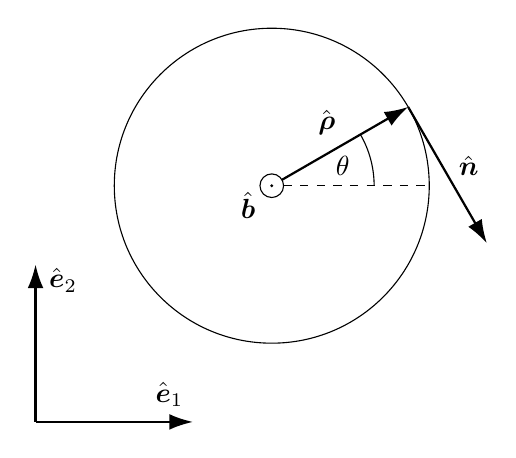
\begin{tikzpicture}
\def\r{2};
\def\th{30};
\coordinate (M) at (3,3);
% draw e1, e2 coordinate system
\draw[-{Latex[length=3mm,width=2mm]},thick] (0,0) -- (\r,0);
\draw[-{Latex[length=3mm,width=2mm]},thick] (0,0) -- (0,\r);
\node at (\r-0.3,0.35) {$\uv{e}_1$};
\node at (0.35,\r-0.2) {$\uv{e}_2$};
% draw circle
\draw (M) circle (\r cm);
% draw rho vector
\draw[-{Latex[length=3mm,width=2mm]},thick] ($(M) + ({0.15*cos(\th)},{0.15*sin(\th)})$) -- ($(M) + ({\r*cos(\th)},{\r*sin(\th)})$);
% draw n vector
\draw[-{Latex[length=3mm,width=2mm]},thick] ($(M) + ({\r*cos(\th)},{\r*sin(\th)})$) -- ($(M) + ({\r*cos(\th)},{\r*sin(\th)}) + ({\r*sin(\th)},{-\r*cos(\th)})$);
% draw angle
\draw[dashed] ($(M) + (0.15,0)$) -- ($(M) + (\r,0)$);
\draw ($(M) + (1.3,0)$) arc (0:\th:13mm);
% draw b vector (out of plane) in the center
\draw (M) circle (1.5mm);
\fill (M) circle (0.2mm);
% vector names
\node at ($(M) - (0.3,0.25)$) {$\uv{b}$};
\node at ($(M) + (0.7,0.8)$) {$\uv{\rho}$};
\node at ($(M) + (2.5,0.25)$) {$\uv{n}$};
\node at ($(M) + (0.9,0.25)$) {$\theta$};
\end{tikzpicture}
\caption{Definition of the trihedron $\uv{\rho}, \uv{b}, \uv{n}$ and the angle $\theta$.}
\label{fig:trihedron}
\end{figure}

By \eqref{eq:trans_gc_r} and \eqref{eq:trans_gc_v} only the transformation $(\rvgc,v_\subparallel,\mu,\theta) \rightarrow (\rv, \vec{v})$ is explicitly defined. It is not obvious that this transformation is invertible for arbitrary magnetic fields $\vec{B} \neq 0$, but for the further discussion we simply assume it is.

In this new coordinate system the phase space Lagrangian becomes
\begin{align}
\PSL(\rvgc,v_\subparallel,\mu,\theta,\dot{\rvgc},\dot{v}_\subparallel,\dot{\mu},\dot{\theta},t) &= \left(mv_{\scriptscriptstyle\subparallel}\,\uv{b}(\rvgc,t) + \sqrt{2B(\rvgc,t)m\mu}\;\uv{n}(\rvgc,\theta,t) + \frac{q}{c}\vec{A}(\rv(\rvgc,\mu,\theta,t),t)\right) \nonumber\\
&\quad\cdot\dv{t}\left[\rvgc + \vec{\rho}(\rvgc,\mu,\theta,t)\right] - \frac{m v_\subparallel^2}{2} - \mu B(\rvgc,t) \nonumber\\
&\quad  - q\,\Phi(\rv(\rvgc,\mu,\theta,t),t) \ , \label{eq:psl_emfield_newcoords}
\end{align}
where $\vec{\rho}(\rvgc,\mu,\theta,t) := \rho_g(\rvgc,\mu,t)\,\uv{\rho}(\rvgc,\theta,t) = \rv-\rvgc$.


\subsection{Simplification of the Phase Space Lagrangian}
The Lagrangian given by \eqref{eq:psl_emfield_newcoords} is still the exact phase space Lagrangian for a charged particle in an electromagnetic field with $\vec{B} \neq 0$ (otherwise the transformation would not be defined). 

As a first approximation we expand the potentials $\Phi$ and $\vec{A}$, which are not exactly known as functions of the new coordinates, into Taylor series,
\begin{align*}
\Phi(\rv) &= \Phi(\rvgc) + \vec{\rho}\cdot\bnabla\Phi(\rvgc) + (\vec{\rho}\cdot\bnabla)^2\Phi(\rvgc)  + \order{\rho^3} \ , \\
\vec{A}(\rv) &= \vec{A}(\rvgc) + (\vec{\rho}\cdot\bnabla)\vec{A}(\rvgc) + (\vec{\rho}\cdot\bnabla)^2\vec{A}(\rvgc) + \order{\rho^3} \ .
\end{align*}
The gradients are in principle taken with respect to $\rv$, but since
\begin{equation*}
\pdv{\rv}{\rvgc} = 1
\end{equation*}
they can just as well be taken with respect to $\rvgc$.

Cutting off the Taylor series after the order $\rho$ leads to the Lagrangian
\begin{align*}
\PSL &= mv_\subparallel \uv{b}\cdot\dot{\rvgc} + \sqrt{2Bm\mu}\;\uv{n}\cdot\dot{\rvgc} + \frac{q}{c}\vec{A}(\rvgc)\cdot\dot{\rvgc} + \frac{q}{c}\dot{\rvgc}\cdot(\vec{\rho}\cdot\bnabla)\vec{A}(\rvgc)\\
& + mv_\subparallel\,\uv{b}\cdot\dot{\vec{\rho}} + \sqrt{2Bm\mu}\,\uv{n}\cdot\dot{\vec{\rho}} \\
& + \frac{q}{c}\vec{A}\cdot\dot{\vec{\rho}} + \frac{q}{c}\dot{\vec{\rho}}\cdot(\vec{\rho}\cdot\bnabla)\vec{A}(\rvgc) \\
& - \frac{m v_\subparallel^2}{2} - \mu B - q\Phi(\rvgc) - q\vec{\rho}\cdot\bnabla\Phi(\rvgc) \ ,
\end{align*}
where the orthogonality of $\uv{b}$, $\uv{n}$ and $\uv{\rho}$ was used. The dependence on the old variable $\rv$ is thereby completely eliminated -- Everything is evaluated at the guiding center position $\rvgc$.

In the next step the Lagrangian is simplified by taking advantage of the gauge invariance (see section \ref{sec:gauge}). Rewriting
\begin{align*}
\vec{A}(\rvgc,t)\cdot\dot{\vec{\rho}} &= \dv{t}\left(\vec{A}(\rvgc,t)\cdot\vec{\rho}\right) - \dv{t}\vec{A}(\rvgc,t)\cdot\vec{\rho} \\
&= \dv{t}\left(\vec{A}(\rvgc,t)\cdot\vec{\rho}\right) - \vec{\rho}\cdot\pdv{\vec{A}(\rvgc,t)}{t} - \vec{\rho}\cdot(\dot{\rvgc}\cdot\bnabla)\vec{A}(\rvgc,t)
\end{align*}
and excluding the total derivative yields
\begin{align}
\PSL &= mv_\subparallel \uv{b}\cdot\dot{\rvgc} + \sqrt{2Bm\mu}\;\uv{n}\cdot\dot{\rvgc} + \frac{q}{c}\vec{A}\cdot\dot{\rvgc} \nonumber\\
& + mv_\subparallel\,\uv{b}\cdot\dot{\vec{\rho}} + \sqrt{2Bm\mu}\,\uv{n}\cdot\dot{\vec{\rho}} \\
& + \frac{q}{c}\dot{\rvgc}\cdot(\vec{\rho}\cdot\bnabla)\vec{A} - \frac{q}{c}\vec{\rho}\cdot(\dot{\rvgc}\cdot\bnabla)\vec{A} - \frac{q}{c}\vec{\rho}\cdot\pdv{\vec{A}}{t} - q\vec{\rho}\cdot\bnabla\Phi \nonumber\\
& + \frac{q}{c}\dot{\vec{\rho}}\cdot(\vec{\rho}\cdot\bnabla)\vec{A} - \frac{m v_\subparallel^2}{2} - \mu B - q\Phi  \ . \label{eq:psl_newcoords_gauge1}
\end{align}
The third line of \eqref{eq:psl_newcoords_gauge1} can be further simplified by noticing that
\begin{equation*}
-\frac{q}{c}\vec{\rho}\cdot\pdv{\vec{A}}{t} - q\vec{\rho}\cdot\bnabla\Phi = q\vec{\rho}\cdot\left(-\frac{1}{c}\pdv{\vec{A}}{t}-\bnabla\Phi\right) = q\vec{\rho}\cdot\vec{E}
\end{equation*}
and
\begin{align*}
&\dot{\rvgc}\cdot(\vec{\rho}\cdot\bnabla)\vec{A} - \vec{\rho}\cdot(\dot{\rvgc}\cdot\bnabla)\vec{A} = \dot{\rgc}_i\rho_j\partial_jA_i - \rho_i\dot{\rgc}_j\partial_jA_i \\
&= \dot{\rgc}_l\rho_m(\delta_{il}\delta_{jm}-\delta_{im}\delta_{jl})\partial_jA_i = \varepsilon_{lmk}\dot{\rgc}_l\rho_m\varepsilon_{ijk}\partial_jA_i = (\dot{\rvgc}\times\vec{\rho})\cdot(-\bnabla\times\vec{A}) \\
&= (\vec{\rho}\times\dot{\rvgc})\cdot\vec{B} = \vec{\rho}\cdot(\dot{\rvgc}\times\vec{B}) \ ,
\end{align*}
resulting in
\begin{align}
\PSL &= mv_\subparallel \uv{b}\cdot\dot{\rvgc} + \sqrt{2Bm\mu}\;\uv{n}\cdot\dot{\rvgc} + \frac{q}{c}\vec{A}\cdot\dot{\rvgc} \nonumber\\
& + mv_\subparallel\,\uv{b}\cdot\dot{\vec{\rho}} + \sqrt{2Bm\mu}\,\uv{n}\cdot\dot{\vec{\rho}} \\
& + \frac{q}{c}\vec{\rho}\cdot(\dot{\rvgc}\times\vec{B}) + q\vec{\rho}\cdot\vec{E} - \frac{m v_\subparallel^2}{2} - \mu B - q\Phi \nonumber\\
&+ \frac{q}{c}\dot{\vec{\rho}}\cdot(\vec{\rho}\cdot\bnabla)\vec{A} \ . \label{eq:psl_newcoords_gauge2}
\end{align}

For the term
\begin{equation*}
\dot{\vec{\rho}}\cdot(\vec{\rho}\cdot\bnabla)\vec{A}
\end{equation*}
we use the gauge invariance again and write
\begin{align*}
\dot{\vec{\rho}}\cdot(\vec{\rho}\cdot\bnabla)\vec{A} &= \frac12\left[\dot{\vec{\rho}}\cdot(\vec{\rho}\cdot\bnabla)\vec{A} + \vec{\rho}\cdot(\dot{\vec{\rho}}\cdot\bnabla)\vec{A}\right] + \frac12\left[\dot{\vec{\rho}}\cdot(\vec{\rho}\cdot\bnabla)\vec{A} - \vec{\rho}\cdot(\dot{\vec{\rho}}\cdot\bnabla)\vec{A}\right] \\
&= \frac12\left[\dv{t}(\vec{\rho}\cdot(\vec{\rho}\cdot\bnabla)\vec{A}) - \vec{\rho}\cdot(\vec{\rho}\cdot\bnabla)\dot{\vec{A}}\right] + \frac12(\vec{\rho}\times\dot{\vec{\rho}})\cdot\vec{B} \ ,
\end{align*}
where the second term was treated analogously to the previous calculation. Again omitting the total derivative yields
\begin{align}
\PSL &= mv_\subparallel \uv{b}\cdot\dot{\rvgc} + \sqrt{2Bm\mu}\;\uv{n}\cdot\dot{\rvgc} + \frac{q}{c}\vec{A}\cdot\dot{\rvgc} \nonumber\\
& + mv_\subparallel\,\uv{b}\cdot\dot{\vec{\rho}} + \sqrt{2Bm\mu}\,\uv{n}\cdot\dot{\vec{\rho}} \nonumber\\
& + \frac{q}{c}\vec{\rho}\cdot(\dot{\rvgc}\times\vec{B}) + q\vec{\rho}\cdot\vec{E} - \frac{m v_\subparallel^2}{2} - \mu B \nonumber\\
& - q\Phi - \frac12\frac{q}{c}\vec{\rho}\cdot(\vec{\rho}\cdot\bnabla)\dot{\vec{A}} + \frac12\frac{q}{c}(\vec{\rho}\times\dot{\vec{\rho}})\cdot\vec{B} \ . \label{eq:psl_newcoords_gauge3}
\end{align}

The last term can be rewritten as
\begin{align*}
\frac12\frac{q}{c}(\vec{\rho}\times\dot{\vec{\rho}})\cdot\vec{B} &= \frac12\frac{q}{c}\rho_g B \left(\uv{b}\times\uv{\rho}\right)\cdot\dot{\vec{\rho}} = -\frac12\sqrt{2Bm\mu}\,\uv{n}\cdot\dot{\vec{\rho}}
\end{align*}
where the Larmor radius \eqref{eq:larmor_radius} was inserted in the last step, and the Lagrangian reads
\begin{align}
\PSL &= mv_\subparallel \uv{b}\cdot\dot{\rvgc} + \sqrt{2Bm\mu}\;\uv{n}\cdot\dot{\rvgc} + \frac{q}{c}\vec{A}\cdot\dot{\rvgc} \nonumber\\
& + mv_\subparallel\,\uv{b}\cdot\dot{\vec{\rho}} + \frac12\sqrt{2Bm\mu}\;\uv{n}\cdot\dot{\vec{\rho}} \nonumber\\
& + \frac{q}{c}\vec{\rho}\cdot(\dot{\rvgc}\times\vec{B}) + q\vec{\rho}\cdot\vec{E} - \frac{m v_\subparallel^2}{2} - \mu B \nonumber\\
& - q\Phi - \frac12\frac{q}{c}\vec{\rho}\cdot(\vec{\rho}\cdot\bnabla)\dot{\vec{A}} \ . \label{eq:psl_newcoords_gauge4}
\end{align}

The term containing $\uv{n}\cdot\dot{\vec{\rho}}$ can be further evaluated to
\begin{align*}
\frac12\sqrt{2Bm\mu}\,\uv{n}\cdot\dot{\vec{\rho}} = \frac12\sqrt{2Bm\mu}\,\uv{n}\cdot\left(\rho_g\dot{\uv{\rho}} + \dot{\rho}_g\uv{\rho}\right) = \frac12\sqrt{2Bm\mu}\,\rho_g\,\uv{n}\cdot\dot{\uv{\rho}} = \frac{c}{q}m\mu\,\uv{n}\cdot\dot{\uv{\rho}}
\end{align*}
and similarly for $\uv{b}\cdot\dot{\vec{\rho}}$, yielding
\begin{align}
\PSL &= mv_\subparallel \uv{b}\cdot\dot{\rvgc} + \sqrt{2Bm\mu}\;\uv{n}\cdot\dot{\rvgc} + \frac{q}{c}\vec{A}\cdot\dot{\rvgc} \nonumber\\
& + mv_\subparallel\rho_g\,\uv{b}\cdot\dot{\uv{\rho}} + \frac{c}{q}m\mu\;\uv{n}\cdot\dot{\uv{\rho}} \nonumber\\
& + q\vec{\rho}\cdot\left(\vec{E} + \frac{1}{c}\dot{\rvgc}\times\vec{B}\right) - \frac{m v_\subparallel^2}{2} - \mu B \nonumber\\
& - q\Phi - \frac12\frac{q}{c}\vec{\rho}\cdot(\vec{\rho}\cdot\bnabla)\dot{\vec{A}} \ . \label{eq:psl_newcoords_gauge5}
\end{align}

The time derivative of $\uv{\rho}$ is given by
\begin{equation*}
    \dv{t}\uv{\rho}(\rvgc,\theta,t) = \pdv{\uv{\rho}}{t} + \dot{\theta}\pdv{\uv{\rho}}{\theta} + \left(\dot{\rvgc}\cdot\bnabla\right)\uv{\rho} = \pdv{\uv{\rho}}{t} + \left(\dot{\rvgc}\cdot\bnabla\right)\uv{\rho} - \dot{\theta}\uv{n} \ ,
\end{equation*}
which, when inserted into the Lagrangian \eqref{eq:psl_newcoords_gauge5}, leads to
\begin{align}
\PSL&(\rvgc,v_\subparallel,\mu,\theta,\dot{\rvgc},\dot{v}_\subparallel,\dot{\mu},\dot{\theta},t) = mv_\subparallel \uv{b}(\rvgc,t)\cdot\dot{\rvgc} + \sqrt{2B(\rvgc,t)m\mu}\;\uv{n}(\rvgc,\theta,t)\cdot\dot{\rvgc} + \frac{q}{c}\vec{A}(\rvgc,t)\cdot\dot{\rvgc} \nonumber\\
& + mv_\subparallel\rho_g(\rvgc,\mu,t)\,\uv{b}(\rvgc,t)\cdot\left(\pdv{t} +  \dot{\rvgc}\cdot\bnabla\right)\uv{\rho}(\rvgc,\theta,t) + \frac{c}{q}m\mu\;\uv{n}(\rvgc,\theta,t)\cdot\left(\pdv{t} +  \dot{\rvgc}\cdot\bnabla\right)\uv{\rho}(\rvgc,\theta,t) \nonumber\\
& - \frac{c}{q}m\mu\dot{\theta} + q\vec{\rho}(\rvgc,\mu,\theta,t)\cdot\left(\vec{E}(\rvgc,t) + \frac{1}{c}\dot{\rvgc}\times\vec{B}(\rvgc,t)\right) - \frac{m v_\subparallel^2}{2} - \mu B(\rvgc,t) \nonumber\\
& - q\Phi(\rvgc,t) - \frac12\frac{q}{c}\vec{\rho}(\rvgc,\mu,\theta,t)\cdot\big(\vec{\rho}(\rvgc,\mu,\theta,t)\cdot\bnabla\big)\dot{\vec{A}}(\rvgc,t) \ . \label{eq:psl_newcoords_gauge6}
\end{align}

\subsection{Dimensionless Quantities and Ordering}

Now we introduce dimensionless coordinates by defining the typical scales $R_0$ for length (system size), $v_0$ for velocity (particle velocity), $m_0$ for mass (particle mass) and $B_0$ for magnetic field (external field). A typical scale for $\mu$ is then given by
\begin{equation*}
\mu_0 B_0 = m_0 v_0^2 \implies \mu_0 = \frac{m_0v_0^2}{B_0} \ ,
\end{equation*}
and the corresponding time scale is
\begin{equation*}
t_0 = \frac{R_0}{v_0} \ .
\end{equation*}
Since the typical Larmor radius is assumed to be much smaller than the system size, the quantity
\begin{equation}
\varepsilon := \frac{\rho_0}{R_0} = \frac{v_0}{\omega_0R_0} = \frac{m_0 c v_0}{eB_0 R_0}
\end{equation}
is small and will be used as an \emph{ordering parameter}, i.e. the relative magnitude of terms is indicated by their order in $\varepsilon$. Here $e$ is the elementary charge.

In these units and with $q=Ze$ the Lagrangian \eqref{eq:psl_newcoords_gauge6} becomes
\begin{align}
\frac{\PSL}{m_0v_0^2} &= \frac{m}{m_0}\frac{v_\subparallel}{v_0} \uv{b}\cdot\frac{\dot{\rvgc}}{v_0} + \underbrace{\sqrt{\frac{B_0m_0\mu_0}{m_0^2v_0^2}}}_{=1}\sqrt{2\frac{B}{B_0}\frac{m}{m_0}\frac{\mu}{\mu_0}}\;\uv{n}\cdot\frac{\dot{\rvgc}}{v_0} + Z\underbrace{\frac{e}{c}\frac{B_0R_0v_0}{m_0v_0^2}}_{=\varepsilon^{-1}}\frac{\vec{A}}{B_0R_0}\cdot\frac{\dot{\rvgc}}{v_0} \nonumber\\ 
& + \frac{1}{Z}\underbrace{\frac{c}{e}\frac{v_0}{R_0}\sqrt{\frac{m_0\mu_0}{B_0v_0^2}}}_{=\varepsilon}\frac{m}{m_0}\frac{v_\subparallel}{v_0}\sqrt{2\frac{m}{m_0}\frac{\mu}{\mu_0}\frac{B_0}{B}}\;\uv{b}\cdot\left(t_0\pdv{t} + \frac{\dot{\rvgc}}{v_0}\cdot R_0\bnabla\right)\uv{\rho}  \nonumber\\
& + \frac{1}{Z}\underbrace{\frac{c}{e}\frac{\mu_0}{R_0v_0}}_{=\varepsilon}\frac{m}{m_0}\frac{\mu}{\mu_0}\;\uv{n}\cdot\left(t_0\pdv{t} + \frac{\dot{\rvgc}}{v_0}\cdot R_0\bnabla\right)\uv{\rho} \nonumber\\
& - \frac{1}{Z}\underbrace{\frac{c}{e}\frac{\mu_0}{v_0R_0}}_{=\varepsilon}\;\frac{m}{m_0}\frac{\mu}{\mu_0}t_0\dot{\theta} + \underbrace{\sqrt{\frac{\mu_0B_0}{m_0v_0^2}}}_{=1} Z\frac{e}{c}\sqrt{2\frac{m}{m_0}\frac{\mu}{\mu_0}\frac{B_0}{B}}\,\uv{\rho}\cdot\left(\frac{c\vec{E}}{v_0B_0}+\frac{\dot{\rvgc}}{v_0}\times\frac{\vec{B}}{B_0}\right) \nonumber\\
& - \frac12\frac{m}{m_0}\frac{v_\subparallel^2}{v_0^2} - \underbrace{\frac{\mu_0B_0}{m_0v_0^2}}_{=1} \frac{\mu}{\mu_0} \frac{B}{B_0} - Z\underbrace{\frac{e}{c}\frac{B_0R_0}{m_0v_0}}_{=\varepsilon^{-1}} \frac{\Phi c}{v_0B_0R_0} \nonumber \\
& - \frac{1}{Z}\underbrace{\frac{c}{e}\frac{\mu_0}{R_0v_0}}_{=\varepsilon} \frac{m}{m_0}\frac{\mu}{\mu_0}\frac{B_0}{B}\uv{\rho}\cdot(\uv{\rho}\cdot R_0\bnabla)\frac{\dot{\vec{A}}t_0}{B_0R_0} \ . \label{eq:psl_newcoords_dimless0}
\end{align}

From here on we will omit the quantities with index 0 and just keep in mind that, unless stated otherwise, everything is measured in these units. Hence the Lagrangian reads
\begin{align}
\PSL &= mv_\subparallel \uv{b}\cdot\dot{\rvgc} + \sqrt{2Bm\mu}\;\uv{n}\cdot\dot{\rvgc} + \varepsilon^{-1}Z\vec{A}\cdot\dot{\rvgc} + \varepsilon \frac{mv_\subparallel}{Z} \sqrt{\frac{2m\mu}{B}}\,\uv{b}\cdot\left(\partial_t+\dot{\rvgc}\cdot\bnabla\right)\uv{\rho} \nonumber\\
& + \varepsilon \frac{m\mu}{Z}\;\uv{n}\cdot\left(\partial_t+\dot{\rvgc}\cdot\bnabla\right)\uv{\rho} - \varepsilon \frac{m\mu}{Z}\dot{\theta} + \frac{Ze}{c}\sqrt{2Bm\mu}\;\uv{\rho}\cdot\left(\vec{E} + \dot{\rvgc}\times\vec{B}\right) \nonumber\\
& - \frac12mv_\subparallel^2 - \mu B - \varepsilon^{-1} Z\Phi  - \varepsilon \frac{m\mu B}{Z}\uv{\rho}\cdot\left(\uv{\rho}\cdot\bnabla\right)\dot{\vec{A}} \ . \label{eq:psl_newcoords_dimless1}
\end{align}


and finally, up to the order $1$,
\begin{align}
\PSL&(\rvgc,v_\subparallel,\mu,\theta,\dot{\rvgc},\dot{v}_\subparallel,\dot{\mu},\dot{\theta},t)  = \varepsilon^{-1}Z\left(\vec{A}(\rvgc,t)\cdot\dot{\rvgc} - \Phi(\rvgc,t)\right) \nonumber\\
& + mv_\subparallel \uv{b}(\rvgc,t)\cdot\dot{\rvgc} + \sqrt{2B(\rvgc,t)m\mu}\;\uv{n}(\rvgc,\theta,t)\cdot\dot{\rvgc}  \nonumber\\
& + \frac{q}{c}\sqrt{2B(\rvgc,t)m\mu}\,\uv{\rho}(\rvgc,\theta,t)\cdot\left(\vec{E}(\rvgc,t) + \dot{\rvgc}\times\vec{B}(\rvgc,t)\right) - \frac12mv_\subparallel^2 - \mu B(\rvgc,t) \nonumber\\
& - \varepsilon \frac{m\mu}{Z}\dot{\theta} +\order{\varepsilon}  \ . \label{eq:psl_newcoords_dimless_ordered_upto1}
\end{align}

Note that we kept the term $\varepsilon m\mu\dot{\theta}/Z$ although it is formally of order $\varepsilon$. However, the gyro frequency $\dot{\theta}$ is large in our new units, because the unit for frequency is $v_0/R_0$ and the gyro frequency is of order $v_0/\rho_0$. Hence $\dot{\theta}$ is in fact of order $\varepsilon^{-1}$ by definition.


This ordering also justifies the Taylor expansion of the potentials: Since $\vec{\rho}\cdot\bnabla_{\rvgc}$ is already dimensionless, the equations for the expansion stay the same in units of $R_0$,
\begin{align*}
\Phi(\rv) &= \Phi(\rvgc) + \bnabla\Phi(\rvgc)\cdot\vec{\rho} + (\vec{\rho}\cdot\bnabla)^2\Phi(\rvgc) + \order{\rho^3} \ , \\
\vec{A}(\rv) &= \vec{A}(\rvgc) + (\vec{\rho}\cdot\bnabla)\vec{A}(\rvgc) + (\vec{\rho}\cdot\bnabla)^2\vec{A}(\rvgc) + \order{\rho^3} \ .
\end{align*}
All terms of order $\rho^2$ or higher are at least of order $\varepsilon^2$, because the derivatives are assumed to be of order 1 or higher and $\rho$ is of order $\varepsilon$.

\subsection{Gyro Averaging}
The Lagrangian \eqref{eq:psl_newcoords_dimless_ordered_upto1} already contains some approximations, but is still rather complicated. Since we are mainly interested in the motion of the guiding center, we will now average the Lagrangian over one gyro period according to
\begin{equation*}
    \langle x \rangle_g := \frac{1}{2\pi} \int\limits_0^{2\pi} x \dd{\theta} \ .
\end{equation*}
Terms, which do not explicitly depend on $\theta$, are evidently not affected by the averaging. The result of this averaging is called the \emph{guiding center Lagrangian} $\PSL_{gc}$,
\begin{align*}
\PSL_{gc}&(\rvgc,v_\subparallel,\mu,\dot{\rvgc},\dot{v}_\subparallel,\dot{\mu},\dot{\theta},t)  = \varepsilon^{-1}Z\left(\vec{A}(\rvgc,t)\cdot\dot{\rvgc} - \Phi(\rvgc,t)\right) \nonumber\\
& + mv_\subparallel \uv{b}(\rvgc,t)\cdot\dot{\rvgc} + \sqrt{2B(\rvgc,t)m\mu}\;\langle\uv{n}(\rvgc,\theta,t)\rangle_g\cdot\dot{\rvgc}  \nonumber\\
& + \frac{q}{c}\sqrt{2m\mu B(\rvgc,t)}\,\langle\uv{\rho}(\rvgc,\theta,t)\rangle_g\cdot\left(\vec{E}(\rvgc,t) + \dot{\rvgc}\times\vec{B}(\rvgc,t)\right) - \frac12mv_\subparallel^2 - \mu B(\rvgc,t) \nonumber\\
& - \varepsilon \frac{m\mu}{Z}\dot{\theta} +\order{\varepsilon}  \ .
\end{align*}

Both $\uv{n}$ and $\uv{\rho}$ only depend on $\sin\theta$ and $\cos\theta$, hence their averages over a whole period are zero. Therefore the guiding center Lagrangian simply reads
\begin{align*}
\PSL_{gc}(\rvgc,v_\subparallel,\mu,\dot{\rvgc},\dot{v}_\subparallel,\dot{\mu},\dot{\theta},t)  &= \varepsilon^{-1}Z\left(\vec{A}(\rvgc,t)\cdot\dot{\rvgc} - \Phi(\rvgc,t)\right) + mv_\subparallel \uv{b}(\rvgc,t)\cdot\dot{\rvgc} \nonumber\\
&  - \varepsilon \frac{m\mu}{Z}\dot{\theta} - \frac12mv_\subparallel^2 - \mu B(\rvgc,t)  +\order{\varepsilon} \ .
\end{align*}


After transforming back to cgs-units the guiding center Lagrangian up to order 1 in $\varepsilon$ is given by
\begin{align}
    \PSL_{gc}(\rvgc,v_\subparallel,\mu,\dot{\rvgc},\dot{\theta},t)  &= \frac{q}{c}\vec{A}(\rvgc,t)\cdot\dot{\rvgc} - q\Phi(\rvgc,t) + mv_\subparallel \uv{b}(\rvgc,t)\cdot\dot{\rvgc} \nonumber\\
&  - \frac{mc\mu}{q}\dot{\theta} - \frac12mv_\subparallel^2 - \mu B(\rvgc,t)  \ , \label{eq:psl_gc_newcoords_dimless_ordered_averaged_upto1_cgs}
\end{align}
where we have to remember that the first two terms are of order $\varepsilon^{-1}$.

\section{Guiding Center Motion}

\subsection{Parallel Motion}
First we evaluate the Euler-Lagrange equation for the Lagrangian \eqref{eq:psl_gc_newcoords_dimless_ordered_averaged_upto1_cgs} with respect to $v_\subparallel$. Since the Lagrangian does not depend on $\dot{v}_\subparallel$, we simply have
\begin{equation*}
    \pdv{\PSL_{gc}}{v_\subparallel} = m\uv{b}\cdot\dot{\rvgc} - mv_\subparallel = 0
\end{equation*}
and hence
\begin{equation}\label{eq:v_para_result}
    v_\subparallel = \uv{b}\cdot\dot{\rvgc} \ .
\end{equation}
In this approximation, the parallel motion thus consists only of the parallel guiding center motion.

\subsection{Gyration Frequency and First Adiabatic Invariant}
For $\mu$ the Euler-Lagrange equation also turns out to be simple, because the Lagrangian does not depend on $\dot{\mu}$. It reads
\begin{equation*}
    \pdv{\PSL_{gc}}{\mu} = -\frac{mc}{q}\dot{\theta} - B(\rvgc,t) = 0
\end{equation*}
and therefore we have
\begin{equation}\label{eq:theta_dot_omegac}
    \dot{\theta} = -\frac{qB(\rvgc,t)}{mc} = -\omega_c \ .
\end{equation}
As expected, the frequency related to $\theta$ (hence to the gyration) is the cyclotron frequency of the respective particle (the negative sign just comes from opposite definition of $\theta$).

Due to the gyro averaging the coordinate $\theta$ has become cyclic in the Lagrangian \eqref{eq:psl_gc_newcoords_dimless_ordered_averaged_upto1_cgs}. Therefore the corresponding canonical momentum is constant,
\begin{equation}\label{eq:mu_const}
p_\theta = \pdv{\PSL_{gc}}{\dot{\theta}} = -\frac{mc\mu}{q} = const.    
\end{equation}

Thus $\mu$ is a constant of motion and is referred to as the \emph{first adiabatic invariant}, because it is only constant up to the order $\varepsilon^0$. Adiabatic invariants are quantities, that vary slowly compared to the typical time scale of the system.

The term $mc\mu/q$ is sometimes called the \emph{gyro action},
\begin{equation}\label{eq:gyroaction}
    J_\perp = \frac{mc\mu}{q} \ ,
\end{equation}
because up to a factor of $2\pi$ it equals the so called action of the generalized coordinate $\theta$,
\begin{equation*}
    J_\theta := \oint p_\theta \dd{\theta} \ .
\end{equation*}

%With \eqref{eq:v_para_result}, \eqref{eq:theta_dot_omegac}, \eqref{eq:mu_const} and \eqref{eq:gyroaction} the Lagrangian \eqref{eq:psl_gc_newcoords_dimless_ordered_averaged_upto1_cgs} can be rewritten as
%\begin{equation}
%    \PSL_{gc}(\rvgc,\dot{\rvgc},t) = \frac{q}{c}\vec{A}(\rvgc,t)\cdot\dot{\rvgc} - q\Phi(\rvgc,t) + \frac12 m\,(\dot{\rvgc}\cdot\uv{b})^2 - J_\perp\omega_c(\rvgc,t) - \mu B(\rvgc,t) \ , \label{eq:psl_gc_partsolved}
%\end{equation}
%or alternatively, since 

\subsection{Lowest Order Motion - ExB Drift}\label{sec:exb}
The lowest order motion is obtained by only keeping the terms of order $\varepsilon^{-1}$ from the Lagrangian \eqref{eq:psl_gc_newcoords_dimless_ordered_averaged_upto1_cgs},
\begin{equation*}
\PSL_{gc}^{(-1)}(\rvgc,\dot{\rvgc},t) = \frac{q}{c}\vec{A}(\rvgc,t)\cdot\dot{\rvgc} - q\Phi(\rvgc,t) \ .
\end{equation*}
This Lagrangian only depends on $\rvgc$ and $\dot{\rvgc}$ and the corresponding Euler-Lagrange equations read
\begin{equation*}
\pdv{\PSL_{gc}^{(-1)}}{R_k}-\dv{t}\pdv{\PSL_{gc}^{(-1)}}{\dot{R}_k} = \frac{q}{c}\pdv{\vec{A}}{R_k}\cdot{\dot{\rvgc}} - q\pdv{\Phi}{R_k} - \frac{q}{c}\dot{A}_k = 0 \ .
\end{equation*}
Using \begin{equation*}
\dot{A}_k = \pdv{A_k}{t} + (\dot{\rvgc}\cdot\bnabla)A_k
\end{equation*}
yields with Einstein's sum convention
\begin{equation*}
\partial_k{A_j}\dot{R}_j - c\pdv{\Phi}{R_k} - \pdv{A_k}{t} - \dot{R}_j\partial_jA_k = 0 \ ,
\end{equation*}
which can be rewritten as
\begin{align*}
0 &= \dot{R}_j(\delta_{jl}\delta_{km}-\delta_{jm}\delta_{kl})\partial_mA_l - c\pdv{\Phi}{R_k} - \pdv{A_k}{t} \\
&= \dot{R_j}\varepsilon_{ijk}\varepsilon_{ilm}\partial_mA_l - c\pdv{\Phi}{R_k} - \pdv{A_k}{t} \\
&= \varepsilon_{kji}\dot{R}_j(\varepsilon_{iml}\partial_mA_l) - c\pdv{\Phi}{R_k} - \pdv{A_k}{t}   \ .
\end{align*}
In vector notation this result reads
\begin{equation*}
\dot{\rvgc}\times(\bnabla\times\vec{A}) - c\bnabla\Phi - \pdv{\vec{A}}{t} = \dot{\rvgc}\times\vec{B} + c\vec{E} = 0 \ .
\end{equation*}
Now we split the guiding center motion into the part parallel to $\vec{B}$ and a drift part, where according to the result \eqref{eq:v_para_result} the parallel part is simply $v_\subparallel$,
\begin{equation*}
\dot{\rvgc} = v_\subparallel\,\uv{b} + \vec{V}_{\!\!D} \ ,
\end{equation*}
which leads to
\begin{equation*}
\vec{V}_{\!\!D}\times\vec{B} + c\vec{E} = 0 \ .
\end{equation*}
Forming the vector product with $\vec{B}$ from the right results in
\begin{equation*}
(\vec{B}\cdot\vec{V}_{\!\!D})\,\vec{B} - B^2\vec{V}_{\!\!D}  + c\vec{E}\times\vec{B} = 0
\end{equation*}
and since $\vec{B}\cdot\vec{V}_{\!\!D}$ vanishes by construction, we arrive at the well-known \emph{$E\times B$-drift}
\begin{equation*}
\vec{V}_{\!\!E} = c\frac{\vec{E}\times\vec{B}}{B^2} \ .
\end{equation*}

\subsection{Other Drifts}
Now the only task remaining is the evaluation of the Euler-Lagrange equations with respect to $\rvgc$ of the full guiding center Lagrangian up to the order 1 \eqref{eq:psl_gc_newcoords_dimless_ordered_averaged_upto1_cgs}.

The derivative with respect to $\rvgc$ yields
\begin{equation*}
    \pdv{\PSL_{gc}}{R_k} = \frac{q}{c}\dot{\rvgc}\cdot\pdv{\vec{A}}{R_k} - q\pdv{\Phi}{R_k} + mv_\subparallel\pdv{\uv{b}}{R_k}\cdot\dot{\rvgc} - \mu\pdv{B}{R_k}
\end{equation*}

and with respect to $\dot{\rvgc}$
\begin{equation*}
    \pdv{\PSL_{gc}}{\dot{R}_k} = \frac{q}{c}A_k + mv_\subparallel b_k
\end{equation*}

resulting in the Euler-Lagrange equations
\begin{equation*}
    \frac{q}{c}\pdv{\vec{A}}{R_k}\cdot\dot{\rvgc} - q\pdv{\Phi}{R_k} - \frac{q}{c}\dot{A}_k + mv_\subparallel\pdv{R_k}(\uv{b}\cdot\dot{\rvgc}) - \mu\pdv{B}{R_k} - m\dot{v}_\subparallel b_k - mv_\subparallel \dot{b}_k = 0 \ .
\end{equation*}

The first three terms are the same as in section \ref{sec:exb} and in vector notation become
\begin{equation*}
     \frac{q}{c}\pdv{\vec{A}}{R_k}\cdot\dot{\rvgc} - q\pdv{\Phi}{R_k} - \frac{q}{c}\dot{A}_k = \left[\dot{\rvgc}\times\vec{B} + c\vec{E}\right]_k
\end{equation*}
where the subscript $k$ denotes the $k$-th component of the vector. Hence the Euler-Lagrange equations can be written in vector form as follows:
\begin{equation*}
    \dot{\rvgc}\times\vec{B} + c\vec{E} + mv_\subparallel\bnabla(\uv{b}\cdot\dot{\rvgc}) - \mu\bnabla B - m\dot{v}_\subparallel\uv{b} - mv_\subparallel\dot{\uv{b}} = 0 \ .
\end{equation*}
In the last term the time derivative of $\uv{b}$ can be expanded using the chain rule,
\begin{equation*}
    \dv{t}\uv{b}(\rvgc,t) = \pdv{\uv{b}}{t} + \left(\dot{\rvgc}\cdot\bnabla\right)\uv{b} \ .
\end{equation*}

The equation then reads
\begin{equation*}
    \dot{\rvgc}\times\vec{B} + c\vec{E}+ mv_\subparallel\bnabla(\uv{b}\cdot\dot{\rvgc})  - \mu\bnabla B - m\dot{v}_\subparallel\uv{b} - mv_\subparallel\pdv{\uv{b}}{t} - mv_\subparallel\left(\dot{\rvgc}\cdot\bnabla\right)\uv{b} = 0 \ .
\end{equation*}

Now we split the guiding center velocity into a parallel part, the known E$\times$B drift and the remaining drift motion,
\begin{equation*}
    \dot{\rvgc} = v_\subparallel\uv{b} + \vec{V}_{\!\!E} + \vec{V}_{\!\!D} = v_\subparallel\uv{b} + c\frac{\vec{E}\times\vec{B}}{B^2} + \vec{V}_{\!\!D}\ ,
\end{equation*}
resulting in
\begin{align*}
    c\frac{(\vec{E}\times\vec{B})\times\vec{B}}{B^2} + \vec{V}_{\!\!D}\times\vec{B} + c\vec{E} + mv_\subparallel\bnabla v_\subparallel - \mu\bnabla B - m\dot{v}_\subparallel\uv{b} - mv_\subparallel\pdv{\uv{b}}{t} & \\ - mv_\subparallel^2\left(\uv{b}\cdot\bnabla\right)\uv{b} - mv_\subparallel\left(\vec{V}_{\!\!E}\cdot\bnabla\right)\uv{b} - mv_\subparallel\left(\vec{V}_{\!\!D}\cdot\bnabla\right)\uv{b}  &= 0 \ .
\end{align*}
Using the BAC-CAB identity the first term becomes
\begin{equation*}
    c\frac{(\vec{E}\times\vec{B})\times\vec{B}}{B^2} = c\frac{\vec{E}\cdot\vec{B}}{B^2}\vec{B} - c\vec{E}
\end{equation*}
and thus the $c\vec{E}$ terms cancel. Forming the vector product with $\vec{B}$ from the left then yields
\begin{align*}
    \vec{B}\times(\vec{V}_{\!\!D}\times\vec{B}) + mv_\subparallel\vec{B}\times\bnabla v_\subparallel  - \mu\vec{B}\times\bnabla B - mv_\subparallel\vec{B}\times\pdv{\uv{b}}{t}  & \\- mv_\subparallel^2\vec{B}\times\left(\uv{b}\cdot\bnabla\right)\uv{b}  - mv_\subparallel\vec{B}\times\left(\vec{V}_{\!\!E}\cdot\bnabla\right)\uv{b} - mv_\subparallel\vec{B}\times\left(\vec{V}_{\!\!D}\cdot\bnabla\right)\uv{b}  &= 0 \ ,
\end{align*}
where the BAC-CAB rule can be applied again to the first term. With $\vec{V}_{\!\!D}\cdot\vec{B} = 0$ we arrive at
\begin{align*}
    \vec{V}_{\!\!D} &= -mv_\subparallel\frac{\vec{B}\times\bnabla v_\subparallel}{B^2} + \mu\frac{\vec{B}\times\bnabla B}{B^2} + mv_\subparallel\frac{1}{B^2}\left(\vec{B}\times\pdv{\uv{b}}{t}\right) + mv_\subparallel^2\frac{\vec{B}\times(\uv{b}\cdot\bnabla)\uv{b}}{B^2}  \\
    & + mv_\subparallel\frac{\vec{B}\times\left(\vec{V}_{\!\!E}\cdot\bnabla\right)\uv{b}}{B^2} + mv_\subparallel\frac{\vec{B}\times(\vec{V}_{\!\!D}\cdot\bnabla)\uv{b}}{B^2} 
\end{align*}

\begin{thebibliography}{xx}
   \bibitem{littlejohn} Robert G. Littlejohn. Variational principles of guiding centre motion. \emph{J. Plasma Physics} 29(1):111-125, 1983.
   \bibitem{cary} John R. Cary, Alain J. Brizard. Hamiltonian theory of guiding-center motion. \emph{Rev. Mod. Phys.} 81(2):693-738, 2009.
   \bibitem{goldstein} Herbert Goldstein, Charles P. Poole, John L. Safko. \textit{Classical Mechanics}. Addison Wesley, 2002.
\end{thebibliography}

\end{document}

